\documentclass{beamer}
\usepackage[orientation=landscape,size=custom,width=16,height=9,scale=0.5,debug]{beamerposter}
\usepackage[utf8]{inputenc}
\usepackage{caption}
\usepackage{overpic}
\usepackage{pgfplots}
\usepackage{cancel}

\usetheme{default}
\author{Jonathan Lang}
\title{Controlling Phasor Noise Artifacts}
\makeatletter
\makeatother

\definecolor{background}{rgb}{1,1,0.9}

\captionsetup{font=small,labelfont=small}
\captionsetup[figure]{labelformat=empty}

\DeclareMathOperator{\atan}{atan}

\setbeamertemplate{footline}[text line]{%
	\insertshortauthor\hfill\insertshorttitle\hfill\insertframenumber/\inserttotalframenumber%
}

\setbeamertemplate{navigation symbols}{}


\begin{document}
\setbeamercolor{background canvas}{bg=background}

\frame{\titlepage}
\frame{\parbox{\textwidth}{\tableofcontents}}

\section{Background}
\frame{
  \frametitle{Gabor Noise}
  $$
    g(\vec{x}) = \exp\left (\frac{||\vec{x}||}{\sigma^2}\right )\cdot \cos(f\langle\vec{x},\vec{u}\rangle)
  $$
  $$
    G(\vec{x}) = \sum_i g(\vec{x}-\vec{p}_i)
  $$
}

\frame{
  \frametitle{Gabor Noise}
    \begin{figure}
      
\includegraphics[width=0.6\textheight]{../report/images/gaborKernel.png} 
      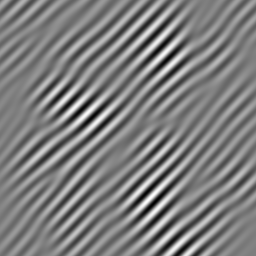
\includegraphics[width=0.6\textheight]{images/gaborNoise.png} 
    \end{figure}
}

\frame{
  \frametitle{Phasor Noise}
	\begin{center}
		\resizebox{0.4\textwidth}{0.3\textheight}{%
			% This file was created by tikzplotlib v0.8.7.
\begin{tikzpicture}

\definecolor{color0}{rgb}{0.12156862745098,0.466666666666667,0.705882352941177}

\begin{axis}[
tick align=outside,
tick pos=left,
x grid style={white!69.01960784313725!black},
xmin=-0.314159265358979, xmax=6.59734457253857,
xtick style={color=black},
y grid style={white!69.01960784313725!black},
ymin=-1.2, ymax=1.2,
ytick style={color=black}
]
\addplot [semithick, color0]
table {%
0 0
0.0125915537218028 0.0950581941535725
0.0251831074436056 0.189057056406544
0.0377746611654083 0.278527630622767
0.0503662148872111 0.360083335427088
0.0629577686090139 0.430547870359788
0.0755493223308167 0.487078234944838
0.0881408760526194 0.527278112945225
0.100732429774422 0.549297134879277
0.113323983496225 0.551911969328585
0.125915537218028 0.534585794538806
0.138507090939831 0.497503446599958
0.151098644661633 0.441580403474179
0.163690198383436 0.368444714657332
0.176281752105239 0.280391989707739
0.188873305827042 0.180314577955981
0.201464859548844 0.0716070678320166
0.214056413270647 -0.0419488310146206
0.22664796699245 -0.156316123044494
0.239239520714253 -0.267346475108794
0.251831074436056 -0.370931129517626
0.264422628157858 -0.463153274742437
0.277014181879661 -0.540436209232926
0.289605735601464 -0.599681687630993
0.302197289323267 -0.638393105282529
0.314788843045069 -0.654778649940693
0.327380396766872 -0.647830214506612
0.339971950488675 -0.617374699600153
0.352563504210478 -0.564095310899782
0.365155057932281 -0.489521538906229
0.377746611654083 -0.395987658836155
0.390338165375886 -0.28656076333056
0.402929719097689 -0.16494049655469
0.415521272819492 -0.0353337511082235
0.428112826541294 0.0976914232800143
0.440704380263097 0.229367606904867
0.4532959339849 0.354899735469947
0.465887487706703 0.469640546720037
0.478479041428506 0.569263298178082
0.491070595150308 0.649925310960285
0.503662148872111 0.708416141250401
0.516253702593914 0.742284663244104
0.528845256315717 0.749940050372186
0.541436810037519 0.730722541982603
0.554028363759322 0.684940949247868
0.566619917481125 0.613875049024917
0.579211471202928 0.519742294555123
0.591803024924731 0.405629590313863
0.604394578646533 0.275392186029185
0.616986132368336 0.133522992709775
0.629577686090139 -0.0150032360715927
0.642169239811942 -0.164905425457286
0.654760793533744 -0.310785172380182
0.667352347255547 -0.447322403611329
0.67994390097735 -0.569470562607585
0.692535454699153 -0.672644121530967
0.705127008420956 -0.752891414761909
0.717718562142758 -0.807046253116252
0.730310115864561 -0.832852489410661
0.742901669586364 -0.829056642129224
0.755493223308167 -0.795464812169942
0.768084777029969 -0.732961407893172
0.780676330751772 -0.643488579744416
0.793267884473575 -0.529986706939259
0.805859438195378 -0.396297721867954
0.818450991917181 -0.24703444919873
0.831042545638983 -0.087420423755736
0.843634099360786 0.0768942148488178
0.856225653082589 0.240034215827018
0.868817206804392 0.396110860651937
0.881408760526194 0.53943607639425
0.894000314247997 0.664731178212403
0.9065918679698 0.767322528547904
0.919183421691603 0.843316815699967
0.931774975413405 0.88974934337138
0.944366529135208 0.904699662128623
0.956958082857011 0.887370030604275
0.969549636578814 0.838123527411424
0.982141190300617 0.758480095965485
0.994732744022419 0.651070340405027
1.00732429774422 0.519548445073849
1.01991585146602 0.368467104986682
1.03250740518783 0.203118773824111
1.04509895890963 0.0293488059438356
1.05769051263143 -0.14665285849101
1.07028206635324 -0.318573981992245
1.08287362007504 -0.480208245324757
1.09546517379684 -0.625681073982249
1.10805672751864 -0.749664795040807
1.12064828124045 -0.847575185444399
1.13323983496225 -0.915742109388353
1.14583138868405 -0.951547852220127
1.15842294240586 -0.953527908992669
1.17101449612766 -0.921430336169035
1.18360604984946 -0.856231276031304
1.19619760357126 -0.760105860283357
1.20878915729307 -0.636355333510882
1.22138071101487 -0.489292848262509
1.23397226473667 -0.324091911808975
1.24656381845847 -0.146602853195812
1.25915537218028 0.0368561239563042
1.27174692590208 0.21972577741308
1.28433847962388 0.39544233880037
1.29693003334569 0.557675103327374
1.30952158706749 0.70055642567278
1.32211314078929 0.818895698113052
1.33470469451109 0.908369445101213
1.3472962482329 0.965680518007689
1.3598878019547 0.988680484147324
1.3724793556765 0.976450635304711
1.38507090939831 0.929338544195658
1.39766246312011 0.848948717611887
1.41025401684191 0.738087572848109
1.42284557056371 0.600664637584768
1.43543712428552 0.441553480889336
1.44802867800732 0.266417364912815
1.46062023172912 0.0815059082367091
1.47321178545093 -0.106569875703265
1.48580333917273 -0.291075998102207
1.49839489289453 -0.465398700538061
1.51098644661633 -0.623283588727542
1.52357800033814 -0.759061974699908
1.53616955405994 -0.867856167028255
1.54876110778174 -0.945756211907299
1.56135266150354 -0.989961627043969
1.57394421522535 -0.998882947395046
1.58653576894715 -0.972199369776313
1.59912732266895 -0.910870388220831
1.61171887639076 -0.81710099453759
1.62431043011256 -0.69426171678522
1.63690198383436 -0.546766419715345
1.64949353755616 -0.379912334786586
1.66208509127797 -0.199688166237796
1.67467664499977 -0.0125572831880586
1.68726819872157 0.174776086949832
1.69985975244337 0.355609134466297
1.71245130616518 0.52348238318984
1.72504285988698 0.672412440719926
1.73763441360878 0.797107124900082
1.75022596733059 0.893155165573548
1.76281752105239 0.957183623102646
1.77540907477419 0.986977357618831
1.78800062849599 0.981556281120425
1.8005921822178 0.941207676440287
1.8131837359396 0.867472515272089
1.8257752896614 0.763086390937921
1.83836684338321 0.631877338298824
1.85095839710501 0.478624382189621
1.86354995082681 0.30888207943578
1.87614150454861 0.128777545846951
1.88873305827042 -0.0552125560111091
1.90132461199222 -0.236496885499052
1.91391616571402 -0.408607561888754
1.92650771943582 -0.565432896562582
1.93909927315763 -0.701436274969635
1.95169082687943 -0.811853283406529
1.96428238060123 -0.892860003050792
1.97687393432304 -0.941706477246064
1.98946548804484 -0.956810656847341
2.00205704176664 -0.937809593715385
2.01464859548844 -0.885566229489252
2.02724014921025 -0.80213175695865
2.03983170293205 -0.690665154399792
2.05242325665385 -0.5553130493742
2.06501481037566 -0.401054500729026
2.07760636409746 -0.233516543757974
2.09019791781926 -0.0587673783408753
2.10278947154106 0.116905143534889
2.11538102526287 0.287221583315385
2.12797257898467 0.446137197651751
2.14056413270647 0.588058217353741
2.15315568642828 0.70804032310817
2.16574724015008 0.801962219720211
2.17833879387188 0.866668168663401
2.19093034759368 0.900074515620679
2.20352190131549 0.901236600619896
2.21611345503729 0.870373912324789
2.22870500875909 0.80885288984015
2.24129656248089 0.719128327703528
2.2538881162027 0.60464584525771
2.2664796699245 0.469709285168563
2.2790712236463 0.3193181564951
2.29166277736811 0.158981290503946
2.30425433108991 -0.00548630490591411
2.31684588481171 -0.168175851993413
2.32943743853351 -0.323298658333174
2.34202899225532 -0.465393624144038
2.35462054597712 -0.589520908469059
2.36721209969892 -0.691434836314347
2.37980365342072 -0.767729953169473
2.39239520714253 -0.815955173857453
2.40498676086433 -0.834692188995636
2.41757831458613 -0.823595637937636
2.43016986830794 -0.78339398099557
2.44276142202974 -0.715851452669854
2.45535297575154 -0.623692897782847
2.46794452947334 -0.510494631654612
2.48053608319515 -0.380545675124821
2.49312763691695 -0.238684751963246
2.50571919063875 -0.0901192635324847
2.51831074436056 0.0597669548660909
2.53090229808236 0.205609958928684
2.54349385180416 0.342258898353928
2.55608540552596 0.464959094410244
2.56867695924777 0.56951844374265
2.58126851296957 0.652451290966201
2.59386006669137 0.71109481082816
2.60645162041317 0.743694010613282
2.61904317413498 0.749452663345499
2.63163472785678 0.728548766191903
2.64422628157858 0.682114437718942
2.65681783530039 0.612181472978304
2.66940938902219 0.521595018631646
2.68200094274399 0.413898966194712
2.69459249646579 0.293197649301515
2.7071840501876 0.16399923600513
2.7197756039094 0.0310468021506602
2.7323671576312 -0.10085656242389
2.74495871135301 -0.22702213707723
2.75755026507481 -0.343043080148332
2.77014181879661 -0.444949050843298
2.78273337251841 -0.529342494071271
2.79532492624022 -0.593511897282471
2.80791647996202 -0.635518248423945
2.82050803368382 -0.654251969434255
2.83309958740562 -0.649458729491969
2.84569114112743 -0.621733713205939
2.85828269484923 -0.572485086889976
2.87087424857103 -0.503868527586087
2.88346580229284 -0.418695713579386
2.89605735601464 -0.320320584684734
2.90864890973644 -0.212507933727315
2.92124046345824 -0.0992894618992211
2.93383201718005 0.0151871982104476
2.94642357090185 0.126810827605593
2.95901512462365 0.231654722076345
2.97160667834546 0.326115197627561
2.98419823206726 0.407035602056987
2.99678978578906 0.471811562128718
3.00938133951086 0.518473970411773
3.02197289323267 0.545747105950525
3.03456444695447 0.553080253099257
3.04715600067627 0.54065219530292
3.05974755439807 0.509348976646551
3.07233910811988 0.460716305503806
3.08493066184168 0.396888885471897
3.09752221556348 0.320499766204217
3.11011376928529 0.234573482480215
3.12270532300709 0.142407271130266
3.13529687672889 0.0474450057770665
3.14788843045069 -0.0468513409411728
3.1604799841725 -0.137127911622604
3.1730715378943 -0.220258251432211
3.1856630916161 -0.293451425794014
3.19825464533791 -0.354345237309469
3.21084619905971 -0.401081450750732
3.22343775278151 -0.432360676462523
3.23602930650331 -0.447475375303195
3.24862086022512 -0.446320300104709
3.26121241394692 -0.429380546480161
3.27380396766872 -0.397698217088403
3.28639552139052 -0.352819477332858
3.29898707511233 -0.296724468946192
3.31157862883413 -0.231743126892391
3.32417018255593 -0.160460395119251
3.33676173627774 -0.0856146438939566
3.34935328999954 -0.0099932475096906
3.36194484372134 0.063670716210238
3.37453639744314 0.132796830310167
3.38712795116495 0.195047240289995
3.39971950488675 0.248404979757598
3.41231105860855 0.291238127652934
3.42490261233036 0.322347809628425
3.43749416605216 0.34099872039969
3.45008571977396 0.346931540320452
3.46267727349576 0.340357320577365
3.47526882721757 0.321934590251207
3.48786038093937 0.292730569605796
3.50045193466117 0.254168434401217
3.51304348838298 0.207963046170392
3.52563504210478 0.156047927646497
3.53822659582658 0.100496509801136
3.55081814954838 0.04344080100492
3.56340970327019 -0.0130093716343657
3.57600125699199 -0.0668435200724932
3.58859281071379 -0.11622125766729
3.60118436443559 -0.159534205872445
3.6137759181574 -0.195457003912485
3.6263674718792 -0.222985864465715
3.638959025601 -0.241463647545238
3.65155057932281 -0.250590976707641
3.66414213304461 -0.250423474191938
3.67673368676641 -0.2413557229859
3.68932524048821 -0.224093053990337
3.70191679421002 -0.199612687488802
3.71450834793182 -0.169116114991086
3.72709990165362 -0.133974878557275
3.73969145537543 -0.095672082037751
3.75228300909723 -0.0557420483619182
3.76487456281903 -0.0157105191597237
3.77746611654083 0.0229623184239004
3.79005767026264 0.0589338902792715
3.80264922398444 0.0910245644357286
3.81524077770624 0.11825477030488
3.82783233142804 0.139872808320142
3.84042388514985 0.155372660326802
3.85301543887165 0.164501533122725
3.86560699259345 0.167257284164263
3.87819854631526 0.163876273058011
3.89079010003706 0.154812539932513
3.90338165375886 0.140709519026723
3.91597320748066 0.122365742242811
3.92856476120247 0.100696165241858
3.94115631492427 0.0766908532435179
3.95374786864607 0.0513727935289858
3.96633942236787 0.0257565583753883
3.97893097608968 0.000809430364319271
3.99152252981148 -0.022583571025186
4.00411408353328 -0.0436495473609662
4.01670563725509 -0.0617515146395787
4.02929719097689 -0.0764054758083574
4.04188874469869 -0.0872904233376383
4.05448029842049 -0.0942512309341971
4.0670718521423 -0.0972946896699962
4.0796634058641 -0.0965792160067317
4.0922549595859 -0.09239899691582
4.10484651330771 -0.0851635318804949
4.11743806702951 -0.0753736765473956
4.13002962075131 -0.063595384068609
4.14262117447311 -0.0504323761077702
4.15521272819492 -0.0364989568935171
4.16780428191672 -0.0223941137386439
4.18039583563852 -0.0086779313637219
4.19298738936032 0.00414880776201476
4.20557894308213 0.0156611505192819
4.21817049680393 0.025522147833591
4.23076205052573 0.0334904147852076
4.24335360424754 0.0394230324203553
4.25594515796934 0.0432739570307497
4.26853671169114 0.0450882941622744
4.28112826541294 0.0449929602856301
4.29371981913475 0.0431843885559648
4.30631137285655 0.0399140317630602
4.31890292657835 0.035472472652339
4.33149448030016 0.0301729684310869
4.34408603402196 0.0243352335151659
4.35667758774376 0.0182702052569422
4.36926914146556 0.0122664459573623
4.38186069518737 0.00657871667087346
4.39445224890917 0.00141912094854379
4.40704380263097 -0.00304893281195329
4.41963535635278 -0.0067138555802979
4.43222691007458 -0.00951614417577486
4.44481846379638 -0.0114459857253874
4.45741001751818 -0.0125385188302366
4.47000157123999 -0.0128671708331396
4.48259312496179 -0.0125355647814982
4.49518467868359 -0.0116685347769502
4.50777623240539 -0.0104028032917441
4.5203677861272 -0.008877859154892
4.532959339849 -0.00722753219793039
4.5455508935708 -0.00557269327976058
4.55814244729261 -0.00401542101424808
4.57073400101441 -0.00263487433716026
4.58332555473621 -0.00148499901787479
4.59591710845801 -0.000594082592378569
4.60850866217982 3.39378104011206e-05
4.62110021590162 0.000416610775250726
4.63369176962342 0.000588830812123586
4.64628332334522 0.000597771883234461
4.65887487706703 0.000497286938700779
4.67146643078883 0.00034218608314409
4.68405798451063 0.000182800918760992
4.69664953823244 6.02132331008576e-05
4.70924109195424 2.47453720455418e-06
4.72183264567604 2.20722190227357e-05
4.73442419939784 0.00011481248062392
4.74701575311965 0.000260194785836915
4.75960730684145 0.000423252788669257
4.77219886056325 0.0005577384010644
4.78479041428506 0.000610434473966726
4.79738196800686 0.000526302814192681
4.80997352172866 0.000254112588803905
4.82256507545046 -0.000247846681116467
4.83515662917227 -0.00100638073452861
4.84774818289407 -0.00202874056693649
4.86033973661587 -0.00329908031130342
4.87293129033768 -0.00477634071410926
4.88552284405948 -0.00639379924548198
4.89811439778128 -0.00806043415484345
4.91070595150308 -0.00966414383002005
4.92329750522489 -0.0110767502373569
4.93588905894669 -0.0121606021034861
4.94848061266849 -0.0127764861206381
4.96107216639029 -0.0127924589537059
4.9736637201121 -0.0120931348774456
4.9862552738339 -0.0105889083931637
4.9988468275557 -0.00822456204973621
5.01143838127751 -0.00498670954890322
5.02402993499931 -0.000909554248465346
5.03662148872111 0.00392149693820512
5.04921304244291 0.00936873639298589
5.06180459616472 0.0152438351009536
5.07439614988652 0.021312425862512
5.08698770360832 0.027301571726527
5.09957925733012 0.0329099478357778
5.11217081105193 0.0378204122454837
5.12476236477373 0.0417144968963697
5.13735391849553 0.044288221446185
5.14994547221734 0.0452685272550308
5.16253702593914 0.0444295527994553
5.17512857966094 0.0416079302937114
5.18772013338274 0.0367162799873782
5.20031168710455 0.0297541154506078
5.21290324082635 0.0208154502618477
5.22549479454815 0.010092512063407
5.23808634826996 -0.00212487977475183
5.25067790199176 -0.0154545371663392
5.26326945571356 -0.0294317897308297
5.27586100943536 -0.0435238822039162
5.28845256315717 -0.0571485110920269
5.30104411687897 -0.0696959153705332
5.31363567060077 -0.0805537386058666
5.32622722432258 -0.0891337083474991
5.33881877804438 -0.0948990420503644
5.35141033176618 -0.097391394987532
5.36400188548798 -0.0962561208035507
5.37659343920979 -0.0912646237781604
5.38918499293159 -0.0823326455225165
5.40177654665339 -0.0695334473165559
5.41436810037519 -0.0531050197444206
5.426959654097 -0.0334506683888756
5.4395512078188 -0.0111325805139654
5.4521427615406 0.0131417367242719
5.46473431526241 0.0385399522458251
5.47732586898421 0.0641318375427611
5.48991742270601 0.088921818362306
5.50250897642781 0.111886065660353
5.51510053014962 0.13201279349195
5.52769208387142 0.148344231304886
5.54028363759322 0.160018594632362
5.55287519131502 0.166310299903002
5.56546674503683 0.166666661975152
5.57805829875863 0.160739380201584
5.59064985248043 0.148409260423365
5.60324140620224 0.129802833192253
5.61583295992404 0.105299806501504
5.62842451364584 0.0755306251538967
5.64101606736764 0.041363786711911
5.65360762108945 0.00388297158094557
5.66619917481125 -0.0356455337550393
5.67879072853305 -0.0758142230588503
5.69138228225485 -0.115123271393063
5.70397383597666 -0.152035296495601
5.71656538969846 -0.185034020734235
5.72915694342026 -0.212684637344056
5.74174849714207 -0.23369352907234
5.75434005086387 -0.246964921988689
5.76693160458567 -0.251652087884559
5.77952315830747 -0.247200837438042
5.79211471202928 -0.23338327124422
5.80470626575108 -0.210320070988702
5.81729781947288 -0.17849000866912
5.82988937319469 -0.138725814448001
5.84248092691649 -0.0921960568996329
5.85507248063829 -0.0403732339758397
5.86766403436009 0.0150111720168029
5.8802555880819 0.0720233787991812
5.8928471418037 0.128593921752637
5.9054386955255 0.182591944593139
5.91803024924731 0.23190452407356
5.93062180296911 0.274518103664867
5.94321335669091 0.308598932141617
5.95580491041271 0.332569341337181
5.96839646413452 0.345176758983638
5.98098801785632 0.3455525386846
5.99357957157812 0.333257995917703
6.00617112529993 0.308315457836421
6.01876267902173 0.271222652144612
6.03135423274353 0.222949358769893
6.04394578646533 0.164915906090193
6.05653734018714 0.0989537867647101
6.06912889390894 0.0272493704430552
6.08172044763074 -0.0477276256107284
6.09431200135254 -0.123308608999131
6.10690355507435 -0.196720662924826
6.11949510879615 -0.265187840597115
6.13208666251795 -0.326035516037204
6.14467821623976 -0.376793885151925
6.15726976996156 -0.415296637883089
6.16986132368336 -0.439770901496619
6.18245287740516 -0.448914787361811
6.19504443112697 -0.441959253620574
6.20763598484877 -0.418711512787519
6.22022753857057 -0.379577849784461
6.23281909229237 -0.325564450360756
6.24541064601418 -0.258255646127323
6.25800219973598 -0.179769830988377
6.27059375345778 -0.0926941627350139
6.28318530717959 -5.38968387752153e-15
};
\end{axis}

\end{tikzpicture}
%
		}
		\resizebox{0.3\textwidth}{0.25\textheight}{%
			$=$
		}\\
	\end{center}
	\only<1>{\resizebox{0.4\textwidth}{0.3\textheight}{\color{background}{test}}}
	\only<2->{
		\resizebox{0.4\textwidth}{0.3\textheight}{%
			% This file was created by tikzplotlib v0.8.7.
\begin{tikzpicture}

\begin{axis}[
tick align=outside,
tick pos=left,
x grid style={white!69.01960784313725!black},
xmin=-0.314159265358979, xmax=6.59734457253857,
xtick style={color=black},
y grid style={white!69.01960784313725!black},
ymin=-1.2, ymax=1.2,
ytick style={color=black}
]
\addplot [semithick, green!50.19607843137255!black]
table {%
0 0.5
0.0125915537218028 0.506295610499228
0.0251831074436056 0.512590222860069
0.0377746611654083 0.518882839102385
0.0503662148872111 0.525172461562514
0.0629577686090139 0.531458093051443
0.0755493223308167 0.537738737012908
0.0881408760526194 0.544013397681393
0.100732429774422 0.550281080240004
0.113323983496225 0.556540790978193
0.125915537218028 0.562791537449306
0.138507090939831 0.569032328627927
0.151098644661633 0.575262175067007
0.163690198383436 0.581480089054728
0.176281752105239 0.587685084771107
0.188873305827042 0.59387617844429
0.201464859548844 0.600052388506522
0.214056413270647 0.606212735749775
0.22664796699245 0.612356243480991
0.239239520714253 0.618481937676936
0.251831074436056 0.624588847138626
0.264422628157858 0.630676003645303
0.277014181879661 0.636742442107946
0.289605735601464 0.642787200722278
0.302197289323267 0.648809321121255
0.314788843045069 0.654807848527015
0.327380396766872 0.660781831902248
0.339971950488675 0.66673032410098
0.352563504210478 0.672652382018741
0.365155057932281 0.678547066742086
0.377746611654083 0.684413443697457
0.390338165375886 0.690250582799354
0.402929719097689 0.696057558597798
0.415521272819492 0.701833450425054
0.428112826541294 0.707577342541599
0.440704380263097 0.713288324281309
0.4532959339849 0.718965490195839
0.465887487706703 0.724607940198178
0.478479041428506 0.730214779705357
0.491070595150308 0.735785119780273
0.503662148872111 0.741318077272635
0.516253702593914 0.746812774958974
0.528845256315717 0.75226834168173
0.541436810037519 0.757683912487365
0.554028363759322 0.763058628763501
0.566619917481125 0.768391638375043
0.579211471202928 0.773682095799289
0.591803024924731 0.778929162259977
0.604394578646533 0.784132005860269
0.616986132368336 0.789289801714649
0.629577686090139 0.794401732079701
0.642169239811942 0.799466986483759
0.654760793533744 0.804484761855403
0.667352347255547 0.809454262650783
0.67994390097735 0.814374700979746
0.692535454699153 0.819245296730758
0.705127008420956 0.824065277694578
0.717718562142758 0.828833879686698
0.730310115864561 0.833550346668491
0.742901669586364 0.838213930867087
0.755493223308167 0.84282389289392
0.768084777029969 0.84737950186196
0.780676330751772 0.851880035501589
0.793267884473575 0.856324780275114
0.805859438195378 0.860713031489895
0.818450991917181 0.865044093410073
0.831042545638983 0.869317279366869
0.843634099360786 0.873531911867459
0.856225653082589 0.877687322702385
0.868817206804392 0.881782853051493
0.881408760526194 0.88581785358839
0.894000314247997 0.889791684583391
0.9065918679698 0.893703716004941
0.919183421691603 0.89755332761951
0.931774975413405 0.901339909089922
0.944366529135208 0.905062860072123
0.956958082857011 0.908721590310366
0.969549636578814 0.912315519730788
0.982141190300617 0.915844078533379
0.994732744022419 0.919306707282325
1.00732429774422 0.9227028569947
1.01991585146602 0.926031989227503
1.03250740518783 0.929293576163032
1.04509895890963 0.932487100692561
1.05769051263143 0.935612056498327
1.07028206635324 0.938667948133803
1.08287362007504 0.941654291102253
1.09546517379684 0.944570611933541
1.10805672751864 0.9474164482592
1.12064828124045 0.95019134888574
1.13323983496225 0.952894873866178
1.14583138868405 0.955526594569795
1.15842294240586 0.958086093750088
1.17101449612766 0.960572965610926
1.18360604984946 0.962986815870886
1.19619760357126 0.965327261825763
1.20878915729307 0.967593932409249
1.22138071101487 0.969786468251759
1.23397226473667 0.971904521737414
1.24656381845847 0.973947757059147
1.25915537218028 0.975915850271948
1.27174692590208 0.977808489344222
1.28433847962388 0.97962537420726
1.29693003334569 0.981366216802814
1.30952158706749 0.983030741128769
1.32211314078929 0.984618683282899
1.33470469451109 0.986129791504707
1.3472962482329 0.987563826215343
1.3598878019547 0.988920560055588
1.3724793556765 0.990199777921897
1.38507090939831 0.991401277000507
1.39766246312011 0.992524866799591
1.41025401684191 0.993570369179456
1.42284557056371 0.994537618380793
1.43543712428552 0.99542646105095
1.44802867800732 0.996236756268249
1.46062023172912 0.996968375564332
1.47321178545093 0.997621202944519
1.48580333917273 0.998195134906211
1.49839489289453 0.998690080455288
1.51098644661633 0.999105961120544
1.52357800033814 0.999442710966125
1.53616955405994 0.999700276601983
1.54876110778174 0.999878617192341
1.56135266150354 0.999977704462165
1.57394421522535 0.999997522701653
1.58653576894715 0.999938068768719
1.59912732266895 0.999799352089494
1.61171887639076 0.999581394656832
1.62431043011256 0.999284231026823
1.63690198383436 0.998907908313314
1.64949353755616 0.998452486180438
1.66208509127797 0.997918036833156
1.67467664499977 0.99730464500581
1.68726819872157 0.996612407948687
1.69985975244337 0.995841435412602
1.71245130616518 0.994991849631496
1.72504285988698 0.994063785303057
1.73763441360878 0.993057389567366
1.75022596733059 0.991972821983564
1.76281752105239 0.990810254504562
1.77540907477419 0.989569871449772
1.78800062849599 0.988251869475887
1.8005921822178 0.986856457545702
1.8131837359396 0.985383856894983
1.8257752896614 0.983834300997392
1.83836684338321 0.982208035527472
1.85095839710501 0.980505318321692
1.86354995082681 0.978726419337575
1.87614150454861 0.976871620610892
1.88873305827042 0.974941216210949
1.90132461199222 0.972935512193962
1.91391616571402 0.970854826554537
1.92650771943582 0.968699489175251
1.93909927315763 0.966469841774348
1.95169082687943 0.964166237851566
1.96428238060123 0.96178904263209
1.97687393432304 0.959338633008646
1.98946548804484 0.956815397481746
2.00205704176664 0.954219736098098
2.01464859548844 0.951552060387172
2.02724014921025 0.948812793295963
2.03983170293205 0.946002369121928
2.05242325665385 0.943121233444134
2.06501481037566 0.940169843052614
2.07760636409746 0.937148665875941
2.09019791781926 0.934058180907046
2.10278947154106 0.930898878127269
2.11538102526287 0.927671258428683
2.12797257898467 0.924375833534674
2.14056413270647 0.921013125918809
2.15315568642828 0.917583668722008
2.16574724015008 0.914088005668009
2.17833879387188 0.910526690977165
2.19093034759368 0.90690028927858
2.20352190131549 0.903209375520582
2.21611345503729 0.899454534879576
2.22870500875909 0.89563636266726
2.24129656248089 0.891755464236244
2.2538881162027 0.887812454884078
2.2664796699245 0.883807959755692
2.2790712236463 0.87974261374429
2.29166277736811 0.875617061390683
2.30425433108991 0.871431956781109
2.31684588481171 0.867187963443522
2.32943743853351 0.862885754242401
2.34202899225532 0.858526011272063
2.35462054597712 0.854109425748527
2.36721209969892 0.849636697899919
2.37980365342072 0.84510853685546
2.39239520714253 0.840525660533033
2.40498676086433 0.835888795525362
2.41757831458613 0.831198676984814
2.43016986830794 0.826456048506845
2.44276142202974 0.821661662012104
2.45535297575154 0.816816277627225
2.46794452947334 0.811920663564305
2.48053608319515 0.806975595999114
2.49312763691695 0.801981858948035
2.50571919063875 0.796940244143759
2.51831074436056 0.791851550909763
2.53090229808236 0.786716586033579
2.54349385180416 0.781536163638883
2.55608540552596 0.776311105056418
2.56867695924777 0.771042238693779
2.58126851296957 0.765730399904069
2.59386006669137 0.760376430853464
2.60645162041317 0.754981180387683
2.61904317413498 0.749545503897415
2.63163472785678 0.744070263182698
2.64422628157858 0.738556326316285
2.65681783530039 0.733004567506015
2.66940938902219 0.727415866956213
2.68200094274399 0.721791110728135
2.69459249646579 0.716131190599492
2.7071840501876 0.710437003923058
2.7197756039094 0.704709453484402
2.7323671576312 0.698949447358755
2.74495871135301 0.69315789876704
2.75755026507481 0.687335725931082
2.77014181879661 0.681483851928032
2.78273337251841 0.675603204544019
2.79532492624022 0.669694716127048
2.80791647996202 0.663759323439184
2.82050803368382 0.657797967508037
2.83309958740562 0.651811593477559
2.84569114112743 0.645801150458201
2.85828269484923 0.639767591376435
2.87087424857103 0.633711872823672
2.88346580229284 0.627634954904601
2.89605735601464 0.621537801084964
2.90864890973644 0.615421378038809
2.92124046345824 0.609286655495226
2.93383201718005 0.603134606084599
2.94642357090185 0.596966205184404
2.95901512462365 0.590782430764567
2.97160667834546 0.584584263232409
2.98419823206726 0.578372685277209
2.99678978578906 0.572148681714404
3.00938133951086 0.565913239329451
3.02197289323267 0.559667346721376
3.03456444695447 0.553411994146035
3.04715600067627 0.547148173359119
3.05974755439807 0.540876877458911
3.07233910811988 0.534599100728837
3.08493066184168 0.528315838479828
3.09752221556348 0.522028086892515
3.11011376928529 0.515736842859293
3.12270532300709 0.509443103826269
3.13529687672889 0.503147867635118
3.14788843045069 0.496852132364882
3.1604799841725 0.490556896173731
3.1730715378943 0.484263157140707
3.1856630916161 0.477971913107486
3.19825464533791 0.471684161520173
3.21084619905971 0.465400899271163
3.22343775278151 0.459123122541089
3.23602930650331 0.452851826640881
3.24862086022512 0.446588005853965
3.26121241394692 0.440332653278625
3.27380396766872 0.434086760670549
3.28639552139052 0.427851318285596
3.29898707511233 0.421627314722791
3.31157862883413 0.415415736767591
3.32417018255593 0.409217569235433
3.33676173627774 0.403033794815596
3.34935328999954 0.396865393915402
3.36194484372134 0.390713344504775
3.37453639744314 0.384578621961191
3.38712795116495 0.378462198915036
3.39971950488675 0.372365045095399
3.41231105860855 0.366288127176328
3.42490261233036 0.360232408623566
3.43749416605216 0.3541988495418
3.45008571977396 0.348188406522442
3.46267727349576 0.342202032491963
3.47526882721757 0.336240676560816
3.48786038093937 0.330305283872953
3.50045193466117 0.324396795455981
3.51304348838298 0.318516148071968
3.52563504210478 0.312664274068919
3.53822659582658 0.306842101232961
3.55081814954838 0.301050552641245
3.56340970327019 0.295290546515598
3.57600125699199 0.289562996076942
3.58859281071379 0.283868809400508
3.60118436443559 0.278208889271865
3.6137759181574 0.272584133043788
3.6263674718792 0.266995432493985
3.638959025601 0.261443673683716
3.65155057932281 0.255929736817302
3.66414213304461 0.250454496102586
3.67673368676641 0.245018819612318
3.68932524048821 0.239623569146537
3.70191679421002 0.234269600095931
3.71450834793182 0.228957761306222
3.72709990165362 0.223688894943583
3.73969145537543 0.218463836361117
3.75228300909723 0.213283413966421
3.76487456281903 0.208148449090237
3.77746611654083 0.203059755856241
3.79005767026264 0.198018141051965
3.80264922398444 0.193024404000886
3.81524077770624 0.188079336435696
3.82783233142804 0.183183722372776
3.84042388514985 0.178338337987896
3.85301543887165 0.173543951493155
3.86560699259345 0.168801323015186
3.87819854631526 0.164111204474638
3.89079010003706 0.159474339466967
3.90338165375886 0.15489146314454
3.91597320748066 0.150363302100081
3.92856476120247 0.145890574251474
3.94115631492427 0.141473988727937
3.95374786864607 0.137114245757599
3.96633942236787 0.132812036556478
3.97893097608968 0.128568043218891
3.99152252981148 0.124382938609317
4.00411408353328 0.120257386255711
4.01670563725509 0.116192040244308
4.02929719097689 0.112187545115922
4.04188874469869 0.108244535763756
4.05448029842049 0.104363637332741
4.0670718521423 0.100545465120424
4.0796634058641 0.0967906244794179
4.0922549595859 0.0930997107214204
4.10484651330771 0.089473309022835
4.11743806702951 0.0859119943319914
4.13002962075131 0.0824163312779917
4.14262117447311 0.0789868740811908
4.15521272819492 0.0756241664653266
4.16780428191672 0.0723287415713167
4.18039583563852 0.0691011218727308
4.19298738936032 0.0659418190929543
4.20557894308213 0.0628513341240586
4.21817049680393 0.0598301569473861
4.23076205052573 0.0568787665558658
4.24335360424754 0.0539976308780724
4.25594515796934 0.0511872067040376
4.26853671169114 0.0484479396128281
4.28112826541294 0.0457802639019025
4.29371981913475 0.0431846025182537
4.30631137285655 0.0406613669913544
4.31890292657835 0.0382109573679102
4.33149448030016 0.0358337621484343
4.34408603402196 0.0335301582256525
4.35667758774376 0.0313005108247494
4.36926914146556 0.0291451734454626
4.38186069518737 0.0270644878060379
4.39445224890917 0.0250587837890516
4.40704380263097 0.023128379389108
4.41963535635278 0.0212735806624247
4.43222691007458 0.0194946816783078
4.44481846379638 0.0177919644725282
4.45741001751818 0.0161656990026077
4.47000157123999 0.014616143105017
4.48259312496179 0.0131435424542979
4.49518467868359 0.0117481305241127
4.50777623240539 0.0104301285502277
4.5203677861272 0.00918974549543761
4.532959339849 0.00802717801643577
4.5455508935708 0.0069426104326345
4.55814244729261 0.00593621469694289
4.57073400101441 0.00500815036850405
4.58332555473621 0.00415856458739783
4.59591710845801 0.00338759205131278
4.60850866217982 0.0026953549941901
4.62110021590162 0.00208196316684423
4.63369176962342 0.00154751381956242
4.64628332334522 0.00109209168668611
4.65887487706703 0.000715768973176767
4.67146643078883 0.00041860534316801
4.68405798451063 0.000200647910506335
4.69664953823244 6.19312312813425e-05
4.70924109195424 2.47729834695898e-06
4.72183264567604 2.22955378347822e-05
4.73442419939784 0.000121382807659443
4.74701575311965 0.000299723398016816
4.75960730684145 0.000557289033874753
4.77219886056325 0.000894038879455994
4.78479041428506 0.00130991954471227
4.79738196800686 0.00180486509378935
4.80997352172866 0.00237879705548055
4.82256507545046 0.00303162443566835
4.83515662917227 0.00376324373175047
4.84774818289407 0.00457353894905033
4.86033973661587 0.00546238161920704
4.87293129033768 0.0064296308205436
4.88552284405948 0.00747513320040916
4.89811439778128 0.00859872299949277
4.91070595150308 0.00980022207810322
4.92329750522489 0.0110794399444124
4.93588905894669 0.0124361737846568
4.94848061266849 0.0138702084952932
4.96107216639029 0.015381316717101
4.9736637201121 0.0169692588712305
4.9862552738339 0.0186337831971856
4.9988468275557 0.0203746257927404
5.01143838127751 0.0221915106557783
5.02402993499931 0.0240841497280518
5.03662148872111 0.0260522429408527
5.04921304244291 0.0280954782625858
5.06180459616472 0.0302135317482407
5.07439614988652 0.0324060675907514
5.08698770360832 0.0346727381742369
5.09957925733012 0.0370131841291139
5.11217081105193 0.0394270343890735
5.12476236477373 0.0419139062499116
5.13735391849553 0.0444734054302046
5.14994547221734 0.0471051261338215
5.16253702593914 0.0498086511142599
5.17512857966094 0.0525835517407998
5.18772013338274 0.0554293880664593
5.20031168710455 0.0583457088977469
5.21290324082635 0.0613320518661968
5.22549479454815 0.0643879435016733
5.23808634826996 0.0675128993074386
5.25067790199176 0.0707064238369674
5.26326945571356 0.0739680107724967
5.27586100943536 0.0772971430053003
5.28845256315717 0.0806932927176747
5.30104411687897 0.0841559214666209
5.31363567060077 0.0876844802692123
5.32622722432258 0.0912784096896337
5.33881877804438 0.0949371399278764
5.35141033176618 0.0986600909100781
5.36400188548798 0.10244667238049
5.37659343920979 0.106296283995058
5.38918499293159 0.110208315416609
5.40177654665339 0.114182146411609
5.41436810037519 0.118217146948507
5.426959654097 0.122312677297615
5.4395512078188 0.12646808813254
5.4521427615406 0.130682720633131
5.46473431526241 0.134955906589927
5.47732586898421 0.139286968510104
5.48991742270601 0.143675219724886
5.50250897642781 0.148119964498411
5.51510053014962 0.152620498138039
5.52769208387142 0.157176107106079
5.54028363759322 0.161786069132912
5.55287519131502 0.166449653331508
5.56546674503683 0.171166120313302
5.57805829875863 0.175934722305422
5.59064985248043 0.180754703269242
5.60324140620224 0.185625299020253
5.61583295992404 0.190545737349217
5.62842451364584 0.195515238144596
5.64101606736764 0.200533013516241
5.65360762108945 0.205598267920299
5.66619917481125 0.210710198285351
5.67879072853305 0.215867994139731
5.69138228225485 0.221070837740023
5.70397383597666 0.22631790420071
5.71656538969846 0.231608361624956
5.72915694342026 0.236941371236499
5.74174849714207 0.242316087512635
5.75434005086387 0.24773165831827
5.76693160458567 0.253187225041026
5.77952315830747 0.258681922727365
5.79211471202928 0.264214880219727
5.80470626575108 0.269785220294643
5.81729781947288 0.275392059801822
5.82988937319469 0.281034509804161
5.84248092691649 0.286711675718691
5.85507248063829 0.2924226574584
5.86766403436009 0.298166549574945
5.8802555880819 0.303942441402201
5.8928471418037 0.309749417200646
5.9054386955255 0.315586556302543
5.91803024924731 0.321452933257914
5.93062180296911 0.327347617981259
5.94321335669091 0.333269675899019
5.95580491041271 0.339218168097752
5.96839646413452 0.345192151472985
5.98098801785632 0.351190678878744
5.99357957157812 0.357212799277722
6.00617112529993 0.363257557892054
6.01876267902173 0.369323996354696
6.03135423274353 0.375411152861374
6.04394578646533 0.381518062323063
6.05653734018714 0.387643756519009
6.06912889390894 0.393787264250225
6.08172044763074 0.399947611493477
6.09431200135254 0.40612382155571
6.10690355507435 0.412314915228893
6.11949510879615 0.418519910945272
6.13208666251795 0.424737824932993
6.14467821623976 0.430967671372072
6.15726976996156 0.437208462550694
6.16986132368336 0.443459209021806
6.18245287740516 0.449718919759996
6.19504443112697 0.455986602318607
6.20763598484877 0.462261262987092
6.22022753857057 0.468541906948556
6.23281909229237 0.474827538437485
6.24541064601418 0.481117160897614
6.25800219973598 0.48740977713993
6.27059375345778 0.493704389500771
6.28318530717959 0.5
};
\end{axis}

\end{tikzpicture}
%
		}
		\resizebox{0.1\textwidth}{0.17\textwidth}{$\cdot$}
	\resizebox{0.4\textwidth}{0.3\textheight}{%
		% This file was created by tikzplotlib v0.8.7.
\begin{tikzpicture}

\definecolor{color0}{rgb}{1,0.647058823529412,0}

\begin{axis}[
tick align=outside,
tick pos=left,
x grid style={white!69.01960784313725!black},
xmin=-0.314159265358979, xmax=6.59734457253857,
xtick style={color=black},
y grid style={white!69.01960784313725!black},
ymin=-1.2, ymax=1.2,
ytick style={color=black}
]
\addplot [semithick, color0]
table {%
0 0
0.0125915537218028 0.18775235688858
0.0251831074436056 0.368826887394913
0.0377746611654083 0.536783276750087
0.0503662148872111 0.685647785787841
0.0629577686090139 0.810125720144247
0.0755493223308167 0.905789747732357
0.0881408760526194 0.969237366565798
0.100732429774422 0.998211922241088
0.113323983496225 0.991682870825204
0.125915537218028 0.949882432421897
0.138507090939831 0.874297331751883
0.151098644661633 0.767615919511385
0.163690198383436 0.633632555254449
0.176281752105239 0.477112652632569
0.188873305827042 0.303623186955117
0.201464859548844 0.119334693442751
0.214056413270647 -0.069198201457674
0.22664796699245 -0.255269909809201
0.239239520714253 -0.432262381198984
0.251831074436056 -0.593880488287519
0.264422628157858 -0.734375926887045
0.277014181879661 -0.848751667069347
0.289605735601464 -0.932939683548695
0.302197289323267 -0.983945643967129
0.314788843045069 -0.99995540892433
0.327380396766872 -0.980399555843794
0.339971950488675 -0.925973631741772
0.352563504210478 -0.838613414564651
0.365155057932281 -0.721426062979792
0.377746611654083 -0.578579603429298
0.390338165375886 -0.415154685083199
0.402929719097689 -0.236963875353874
0.415521272819492 -0.0503449231250294
0.428112826541294 0.138064657255855
0.440704380263097 0.321563663804495
0.4532959339849 0.493625549917947
0.465887487706703 0.648130555389155
0.478479041428506 0.779583369166782
0.491070595150308 0.883308582204505
0.503662148872111 0.955616978688443
0.516253702593914 0.993936751128663
0.528845256315717 0.996904972360875
0.541436810037519 0.964416071054944
0.554028363759322 0.897625586591925
0.566619917481125 0.798909069759153
0.579211471202928 0.671777591050726
0.591803024924731 0.520752861706928
0.604394578646533 0.351206409088038
0.616986132368336 0.169168526464818
0.629577686090139 -0.0188862076525375
0.642169239811942 -0.206269212169196
0.654760793533744 -0.386315797534077
0.667352347255547 -0.552622210112833
0.67994390097735 -0.699273395799838
0.692535454699153 -0.82105338195433
0.705127008420956 -0.913630794963493
0.717718562142758 -0.973712915091404
0.730310115864561 -0.999162789313664
0.742901669586364 -0.989075236761586
0.755493223308167 -0.943809043474829
0.768084777029969 -0.864974201385122
0.780676330751772 -0.755374645404771
0.793267884473575 -0.618908525301567
0.805859438195378 -0.460429559410715
0.818450991917181 -0.285574401444556
0.831042545638983 -0.100562160480009
0.843634099360786 0.0880267953627833
0.856225653082589 0.273484884215892
0.868817206804392 0.449215880396355
0.881408760526194 0.608969523710805
0.894000314247997 0.747063823734919
0.9065918679698 0.858587152326064
0.919183421691603 0.939572936503518
0.931774975413405 0.987140738358912
0.944366529135208 0.999598704178987
0.956958082857011 0.976503738951775
0.969549636578814 0.918677266017292
0.982141190300617 0.828176011336018
0.994732744022419 0.708218851497054
1.00732429774422 0.563072327277766
1.01991585146602 0.397898894717512
1.03250740518783 0.218573310990451
1.04509895890963 0.0314736857185886
1.05769051263143 -0.156745370554417
1.07028206635324 -0.339389432254092
1.08287362007504 -0.509962360775365
1.09546517379684 -0.662397353969627
1.10805672751864 -0.791272725334518
1.12064828124045 -0.892004738243854
1.13323983496225 -0.961010636643384
1.14583138868405 -0.995836073666312
1.15842294240586 -0.995242405889039
1.17101449612766 -0.959250748414519
1.18360604984946 -0.889141223867082
1.19619760357126 -0.787407432009884
1.20878915729307 -0.657667759373395
1.22138071101487 -0.504536683363463
1.23397226473667 -0.333460648201961
1.24656381845847 -0.150524350134018
1.25915537218028 0.0377656782047693
1.27174692590208 0.224712486961983
1.28433847962388 0.403666900850106
1.29693003334569 0.568264011720538
1.30952158706749 0.712649560550225
1.32211314078929 0.831688157066758
1.33470469451109 0.921145931221851
1.3472962482329 0.977841120111175
1.3598878019547 0.999757234384681
1.3724793556765 0.986114779134732
1.38507090939831 0.937398978350501
1.39766246312011 0.855342516857369
1.41025401684191 0.742863913562219
1.42284557056371 0.603963717896072
1.43543712428552 0.443582221456273
1.44802867800732 0.267423745647344
1.46062023172912 0.0817537549178256
1.47321178545093 -0.106823988292069
1.48580333917273 -0.291602300916399
1.49839489289453 -0.466009135012028
1.51098644661633 -0.623841327128607
1.52357800033814 -0.759485227488577
1.53616955405994 -0.868116361814091
1.54876110778174 -0.945871024387923
1.56135266150354 -0.989983699262992
1.57394421522535 -0.99888542193225
1.58653576894715 -0.972259583009414
1.59912732266895 -0.911053189139592
1.61171887639076 -0.817443180620735
1.62431043011256 -0.694759003723921
1.63690198383436 -0.54736419159858
1.64949353755616 -0.38050116559871
1.66208509127797 -0.200104777013047
1.67467664499977 -0.0125912209984597
1.68726819872157 0.175370169542211
1.69985975244337 0.357094133484171
1.71245130616518 0.526117257527
1.72504285988698 0.676427861734174
1.73763441360878 0.802679818179842
1.75022596733059 0.900382697771479
1.76281752105239 0.966061482257538
1.77540907477419 0.997380160910575
1.78800062849599 0.993224815897375
1.8005921822178 0.953743241221785
1.8131837359396 0.880339686105229
1.8257752896614 0.775624909768158
1.83836684338321 0.643323324024211
1.85095839710501 0.488140526365396
1.86354995082681 0.315595935016078
1.87614150454861 0.131826478658904
1.88873305827042 -0.0566316769596525
1.90132461199222 -0.243075602169925
1.91391616571402 -0.420874007846116
1.92650771943582 -0.583703101819523
1.93909927315763 -0.725771508484801
1.95169082687943 -0.842026251837616
1.96428238060123 -0.928332475703131
1.97687393432304 -0.981620509009124
1.98946548804484 -0.999995045403306
2.00205704176664 -0.982802554001015
2.01464859548844 -0.930654523651527
2.02724014921025 -0.8454057139894
2.03983170293205 -0.730088186820147
2.05242325665385 -0.588803464159408
2.06501481037566 -0.426576648562618
2.07760636409746 -0.249177694277256
2.09019791781926 -0.0629161861028908
2.10278947154106 0.12558307489861
2.11538102526287 0.309615697054029
2.12797257898467 0.482636154545267
2.14056413270647 0.63849059346151
2.15315568642828 0.771635707176778
2.16574724015008 0.877335896267606
2.17833879387188 0.951831700543895
2.19093034759368 0.992473512536499
2.20352190131549 0.997815816626628
2.21611345503729 0.967668601994786
2.22870500875909 0.903104120774347
2.24129656248089 0.806418751041167
2.2538881162027 0.681051321066067
2.2664796699245 0.531460799808143
2.2790712236463 0.362967703856067
2.29166277736811 0.181564861529133
2.30425433108991 -0.00629573527023199
2.31684588481171 -0.1939324103688
2.32943743853351 -0.374671451862158
2.34202899225532 -0.542084477387555
2.35462054597712 -0.690217073710916
2.36721209969892 -0.813800578557157
2.37980365342072 -0.908439472196195
2.39239520714253 -0.970767713789965
2.40498676086433 -0.998568462053646
2.41757831458613 -0.990852922101899
2.43016986830794 -0.947895514118295
2.44276142202974 -0.871224112996657
2.45535297575154 -0.763565706102989
2.46794452947334 -0.628749401959493
2.48053608319515 -0.471570239560551
2.49312763691695 -0.297618642242519
2.50571919063875 -0.113081581956386
2.51831074436056 0.0754774740258123
2.53090229808236 0.2613520072906
2.54349385180416 0.43793098039168
2.55608540552596 0.598933972967518
2.56867695924777 0.738634558733734
2.58126851296957 0.852063978455001
2.59386006669137 0.935187864818497
2.60645162041317 0.985049733599181
2.61904317413498 0.999876137537437
2.63163472785678 0.979139742899544
2.64422628157858 0.923578085264181
2.65681783530039 0.83516733744402
2.66940938902219 0.717052022544133
2.68200094274399 0.573433172067158
2.69459249646579 0.409418906968808
2.7071840501876 0.230842756077626
2.7197756039094 0.044056173785027
2.7323671576312 -0.144297363428806
2.74495871135301 -0.327518646878362
2.75755026507481 -0.499091007794826
2.77014181879661 -0.652912097013689
2.78273337251841 -0.783510928472486
2.79532492624022 -0.886242466888264
2.80791647996202 -0.957452838675151
2.82050803368382 -0.99460929001162
2.83309958740562 -0.996390269812422
2.84569114112743 -0.96273243360563
2.85828269484923 -0.894832896518401
2.87087424857103 -0.795106655239023
2.88346580229284 -0.667100693336985
2.89605735601464 -0.51536782497473
2.90864890973644 -0.345304764037486
2.92124046345824 -0.162960178109463
2.93383201718005 0.0251804457201339
2.94642357090185 0.212425471499548
2.95901512462365 0.392115117195591
2.97160667834546 0.557858324519951
2.98419823206726 0.703760071003178
2.99678978578906 0.824631039461573
3.00938133951086 0.916172187500173
3.02197289323267 0.975127652430685
3.03456444695447 0.999400553203966
3.04715600067627 0.988127570606115
3.05974755439807 0.941709653109076
3.07233910811988 0.861797756254539
3.08493066184168 0.751234122781369
3.09752221556348 0.613951191998235
3.11011376928529 0.45483173391243
3.12270532300709 0.279535182752872
3.13529687672889 0.0942963467182446
3.14788843045069 -0.0942963467182339
3.1604799841725 -0.279535182752868
3.1730715378943 -0.454831733912421
3.1856630916161 -0.613951191998226
3.19825464533791 -0.751234122781362
3.21084619905971 -0.861797756254537
3.22343775278151 -0.941709653109072
3.23602930650331 -0.988127570606114
3.24862086022512 -0.999400553203966
3.26121241394692 -0.975127652430687
3.27380396766872 -0.916172187500178
3.28639552139052 -0.824631039461579
3.29898707511233 -0.703760071003181
3.31157862883413 -0.557858324519954
3.32417018255593 -0.392115117195601
3.33676173627774 -0.212425471499552
3.34935328999954 -0.0251804457201447
3.36194484372134 0.162960178109453
3.37453639744314 0.345304764037476
3.38712795116495 0.515367824974727
3.39971950488675 0.667100693336982
3.41231105860855 0.795106655239017
3.42490261233036 0.894832896518399
3.43749416605216 0.962732433605627
3.45008571977396 0.996390269812421
3.46267727349576 0.994609290011621
3.47526882721757 0.957452838675152
3.48786038093937 0.886242466888269
3.50045193466117 0.783510928472492
3.51304348838298 0.652912097013692
3.52563504210478 0.499091007794836
3.53822659582658 0.327518646878373
3.55081814954838 0.144297363428817
3.56340970327019 -0.0440561737850234
3.57600125699199 -0.230842756077616
3.58859281071379 -0.409418906968798
3.60118436443559 -0.573433172067155
3.6137759181574 -0.717052022544126
3.6263674718792 -0.835167337444014
3.638959025601 -0.923578085264176
3.65155057932281 -0.979139742899544
3.66414213304461 -0.999876137537437
3.67673368676641 -0.985049733599183
3.68932524048821 -0.935187864818499
3.70191679421002 -0.852063978455007
3.71450834793182 -0.738634558733742
3.72709990165362 -0.598933972967526
3.73969145537543 -0.437930980391677
3.75228300909723 -0.26135200729061
3.76487456281903 -0.0754774740258231
3.77746611654083 0.113081581956382
3.79005767026264 0.297618642242509
3.80264922398444 0.471570239560542
3.81524077770624 0.628749401959485
3.82783233142804 0.763565706102986
3.84042388514985 0.871224112996651
3.85301543887165 0.947895514118292
3.86560699259345 0.990852922101899
3.87819854631526 0.998568462053647
3.89079010003706 0.970767713789968
3.90338165375886 0.9084394721962
3.91597320748066 0.81380057855716
3.92856476120247 0.690217073710923
3.94115631492427 0.542084477387564
3.95374786864607 0.374671451862168
3.96633942236787 0.193932410368811
3.97893097608968 0.00629573527024277
3.99152252981148 -0.181564861529123
4.00411408353328 -0.362967703856057
4.01670563725509 -0.531460799808134
4.02929719097689 -0.681051321066065
4.04188874469869 -0.806418751041161
4.05448029842049 -0.903104120774342
4.0670718521423 -0.967668601994785
4.0796634058641 -0.997815816626628
4.0922549595859 -0.992473512536499
4.10484651330771 -0.9518317005439
4.11743806702951 -0.877335896267611
4.13002962075131 -0.771635707176781
4.14262117447311 -0.638490593461524
4.15521272819492 -0.482636154545277
4.16780428191672 -0.309615697054029
4.18039583563852 -0.125583074898621
4.19298738936032 0.06291618610288
4.20557894308213 0.249177694277249
4.21817049680393 0.426576648562611
4.23076205052573 0.588803464159399
4.24335360424754 0.730088186820145
4.25594515796934 0.845405713989396
4.26853671169114 0.930654523651525
4.28112826541294 0.982802554001012
4.29371981913475 0.999995045403306
4.30631137285655 0.981620509009126
4.31890292657835 0.928332475703133
4.33149448030016 0.84202625183762
4.34408603402196 0.725771508484801
4.35667758774376 0.583703101819535
4.36926914146556 0.420874007846123
4.38186069518737 0.243075602169932
4.39445224890917 0.0566316769596703
4.40704380263097 -0.131826478658904
4.41963535635278 -0.315595935016078
4.43222691007458 -0.48814052636539
4.44481846379638 -0.643323324024206
4.45741001751818 -0.775624909768147
4.47000157123999 -0.880339686105222
4.48259312496179 -0.953743241221781
4.49518467868359 -0.993224815897374
4.50777623240539 -0.997380160910576
4.5203677861272 -0.966061482257539
4.532959339849 -0.900382697771485
4.5455508935708 -0.802679818179848
4.55814244729261 -0.676427861734179
4.57073400101441 -0.526117257527016
4.58332555473621 -0.357094133484172
4.59591710845801 -0.175370169542211
4.60850866217982 0.0125912209984489
4.62110021590162 0.20010477701304
4.63369176962342 0.380501165598694
4.64628332334522 0.547364191598568
4.65887487706703 0.694759003723914
4.67146643078883 0.817443180620728
4.68405798451063 0.911053189139589
4.69664953823244 0.972259583009413
4.70924109195424 0.99888542193225
4.72183264567604 0.989983699262993
4.73442419939784 0.945871024387926
4.74701575311965 0.868116361814093
4.75960730684145 0.75948522748858
4.77219886056325 0.623841327128607
4.78479041428506 0.466009135012037
4.79738196800686 0.291602300916406
4.80997352172866 0.106823988292087
4.82256507545046 -0.0817537549178078
4.83515662917227 -0.267423745647347
4.84774818289407 -0.443582221456263
4.86033973661587 -0.603963717896066
4.87293129033768 -0.742863913562216
4.88552284405948 -0.85534251685736
4.89811439778128 -0.937398978350498
4.91070595150308 -0.98611477913473
4.92329750522489 -0.999757234384681
4.93588905894669 -0.977841120111176
4.94848061266849 -0.921145931221852
4.96107216639029 -0.831688157066764
4.9736637201121 -0.712649560550233
4.9862552738339 -0.568264011720552
4.9988468275557 -0.40366690085011
5.01143838127751 -0.22471248696198
5.02402993499931 -0.0377656782047801
5.03662148872111 0.150524350134007
5.04921304244291 0.333460648201958
5.06180459616472 0.504536683363447
5.07439614988652 0.657667759373386
5.08698770360832 0.787407432009886
5.09957925733012 0.889141223867079
5.11217081105193 0.959250748414518
5.12476236477373 0.995242405889039
5.13735391849553 0.995836073666313
5.14994547221734 0.961010636643387
5.16253702593914 0.892004738243864
5.17512857966094 0.79127272533452
5.18772013338274 0.662397353969627
5.20031168710455 0.509962360775374
5.21290324082635 0.339389432254102
5.22549479454815 0.156745370554422
5.23808634826996 -0.0314736857185707
5.25067790199176 -0.218573310990439
5.26326945571356 -0.397898894717515
5.27586100943536 -0.56307232727776
5.28845256315717 -0.70821885149705
5.30104411687897 -0.828176011336017
5.31363567060077 -0.918677266017287
5.32622722432258 -0.976503738951773
5.33881877804438 -0.999598704178987
5.35141033176618 -0.987140738358913
5.36400188548798 -0.939572936503518
5.37659343920979 -0.858587152326071
5.38918499293159 -0.747063823734925
5.40177654665339 -0.608969523710811
5.41436810037519 -0.449215880396371
5.426959654097 -0.273484884215906
5.4395512078188 -0.0880267953627817
5.4521427615406 0.10056216048
5.46473431526241 0.285574401444551
5.47732586898421 0.460429559410712
5.48991742270601 0.618908525301555
5.50250897642781 0.755374645404764
5.51510053014962 0.864974201385119
5.52769208387142 0.943809043474827
5.54028363759322 0.989075236761586
5.55287519131502 0.999162789313665
5.56546674503683 0.973712915091406
5.57805829875863 0.913630794963495
5.59064985248043 0.821053381954341
5.60324140620224 0.699273395799838
5.61583295992404 0.552622210112833
5.62842451364584 0.386315797534087
5.64101606736764 0.206269212169203
5.65360762108945 0.0188862076525412
5.66619917481125 -0.169168526464803
5.67879072853305 -0.351206409088027
5.69138228225485 -0.52075286170692
5.70397383597666 -0.67177759105072
5.71656538969846 -0.79890906975915
5.72915694342026 -0.897625586591919
5.74174849714207 -0.964416071054941
5.75434005086387 -0.996904972360875
5.76693160458567 -0.993936751128664
5.77952315830747 -0.955616978688444
5.79211471202928 -0.883308582204505
5.80470626575108 -0.779583369166788
5.81729781947288 -0.648130555389161
5.82988937319469 -0.493625549917951
5.84248092691649 -0.32156366380451
5.85507248063829 -0.138064657255853
5.86766403436009 0.0503449231250195
5.8802555880819 0.236963875353867
5.8928471418037 0.415154685083196
5.9054386955255 0.578579603429286
5.91803024924731 0.721426062979783
5.93062180296911 0.838613414564646
5.94321335669091 0.92597363174177
5.95580491041271 0.980399555843793
5.96839646413452 0.99995540892433
5.98098801785632 0.98394564396713
5.99357957157812 0.932939683548698
6.00617112529993 0.84875166706935
6.01876267902173 0.734375926887056
6.03135423274353 0.593880488287518
6.04394578646533 0.432262381198994
6.05653734018714 0.255269909809209
6.06912889390894 0.0691982014576785
6.08172044763074 -0.119334693442735
6.09431200135254 -0.303623186955105
6.10690355507435 -0.477112652632561
6.11949510879615 -0.633632555254444
6.13208666251795 -0.767615919511382
6.14467821623976 -0.874297331751883
6.15726976996156 -0.949882432421893
6.16986132368336 -0.991682870825203
6.18245287740516 -0.998211922241088
6.19504443112697 -0.969237366565802
6.20763598484877 -0.905789747732357
6.22022753857057 -0.810125720144253
6.23281909229237 -0.685647785787847
6.24541064601418 -0.536783276750092
6.25800219973598 -0.368826887394929
6.27059375345778 -0.187752356888593
6.28318530717959 -1.07793677550431e-14
};
\end{axis}

\end{tikzpicture}
%
	}
	}
}

\frame{
  \frametitle{Phasor Noise}
  \begin{columns}
    \column{0.5\textwidth}
    $$
      G(\vec{x}) = \only<1>{I(\vec{x})}\only<2->{\xcancel{I(\vec{x})}}\cdot\sin(f\langle\vec{x},\vec{u}\rangle + \varphi(\vec{x}))
    $$
    \column{0.5\textwidth}
    \begin{figure}
      \centering
      \only<2->{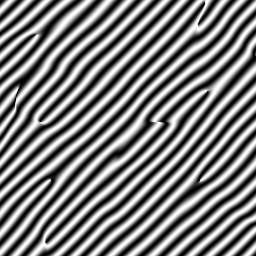
\includegraphics[width=0.6\textheight]{images/phasorSineWave.png}}
    \end{figure}
  \end{columns}
}

\section{Controlling the Artifacts}
\frame{
  \frametitle{$\varphi$}
  \begin{figure}
    \centering
    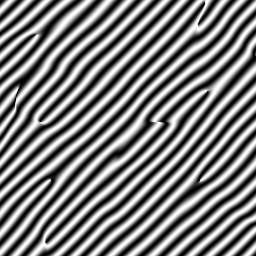
\includegraphics[height=0.6\textheight]{images/phasorSineWave.png}
    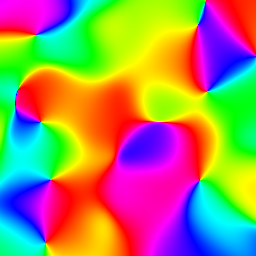
\includegraphics[height=0.6\textheight]{../report/images/phasorPhase.png}
  \end{figure}
}

\subsection{Wobble}
\frame{
  \frametitle{Wobble}
  \begin{figure}
    \centering
    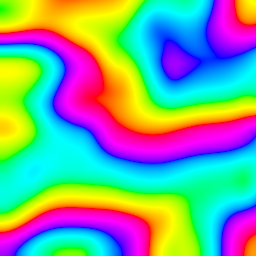
\includegraphics[height=0.6\textheight]{../report/images/wobblePhase.png}
    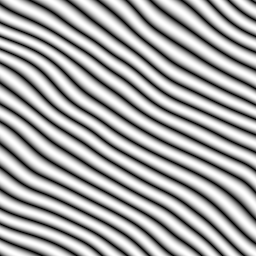
\includegraphics[height=0.6\textheight]{../report/images/wobble.png}
  \end{figure}
}
\subsection{Singularities}
\frame{
  \frametitle{Right Singularity}
  \begin{figure}
    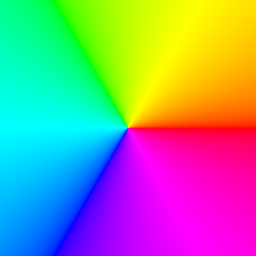
\includegraphics[height=0.6\textheight]{../report/images/rightSingularityPhase.png}
    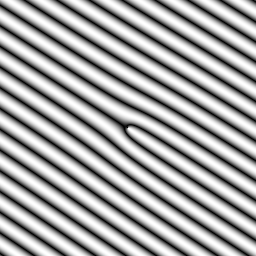
\includegraphics[height=0.6\textheight]{../report/images/rightSingularity.png}
  \end{figure}
}

\frame{
  \frametitle{Left Singularity}
  \begin{figure}
    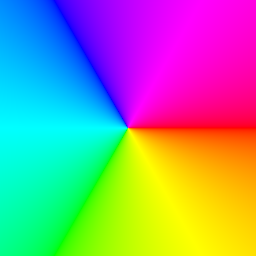
\includegraphics[height=0.6\textheight]{../report/images/leftSingularityPhase.png}
    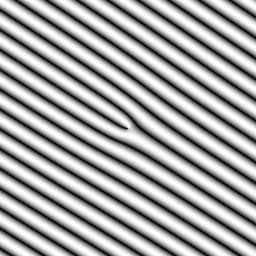
\includegraphics[height=0.6\textheight]{../report/images/leftSingularity.png}
  \end{figure}
}

\frame{
  \frametitle{Formulas}
  \begin{align*}
    r(\vec{x}) &= \atan(\vec{x})\\
    l(\vec{x}) &= -\atan(\vec{x})
  \end{align*}
}

\frame{
  \frametitle{Fading out}
  \begin{figure}
    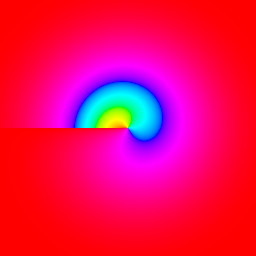
\includegraphics[height=0.6\textheight]{../report/images/fadedPhase.png}
    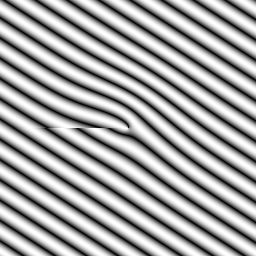
\includegraphics[height=0.6\textheight]{../report/images/fadedPhaseSineWave.png}
  \end{figure}
}

\frame{
  \frametitle{Dual Singularities}
  \begin{figure}
    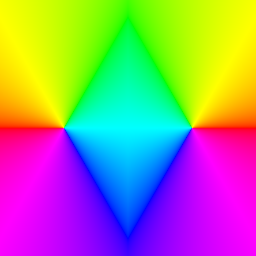
\includegraphics[height=0.6\textheight]{../report/images/dualSingularityPhase.png}
    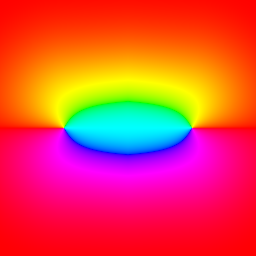
\includegraphics[height=0.6\textheight]{../report/images/dualSingularityFaded.png}
  \end{figure}
}

\frame{
  \frametitle{Dual Singularities}
  \begin{figure}
    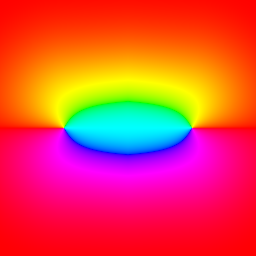
\includegraphics[height=0.6\textheight]{../report/images/dualSingularityFaded.png}
    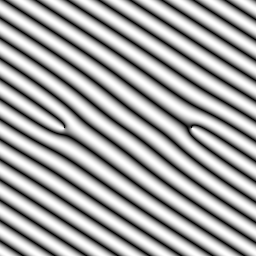
\includegraphics[height=0.6\textheight]{../report/images/dualSingularitySineWave.png}
  \end{figure}
}

\frame{
  \frametitle{Formulas}
  \begin{align*}
    a(\vec{x}) &= \begin{cases}
    \atan(\vec{x}-\vec{s}) - \theta, &\text{if $s$ nearer than $t$}\\
    \pi - \atan(\vec{x}-\vec{t}) + \theta, &\text{otherwise}
    \end{cases}\\
  \uncover<2->{
    b(\vec{x}) &= \begin{cases}
      \exp\left (\frac{d_s^2}{\sigma^2}\right ), &\text{if }d_s < d_t \land d_s < d_l\\
      \exp\left (\frac{d_t^2}{\sigma^2}\right ), &\text{if }d_t < d_s \land d_t < d_l\\
      \exp\left (\frac{d_l^2}{\sigma^2}\right ), &\text{otherwise}\\
    \end{cases}\\
  }
    \uncover<3->{d(\vec{x}) &= ((a(\vec{x})-\pi)\ \mathrm{mod}\ 2\pi)\ b(\vec{x})}
  \end{align*}

}

\subsection{Rips}
\section{Multiple Directions}
\section{Results}

\end{document}
